\section{Evaluation Tasks}
\label{sec:tasks}

\section{Questionnaires and Results}
\label{sec:qs}

\section{Similar Plots}
\label{sec:mutants}

This appendix contains the set of similar plots generated by mutation.  Figure~\ref{fig:query} contains the query plot that the mutations are based on.  The other figures contain the query plot and the mutant.  In the other figures the blue line is the query plot and the green line is the mutation.

\begin{figure}[h!]
    \centering
    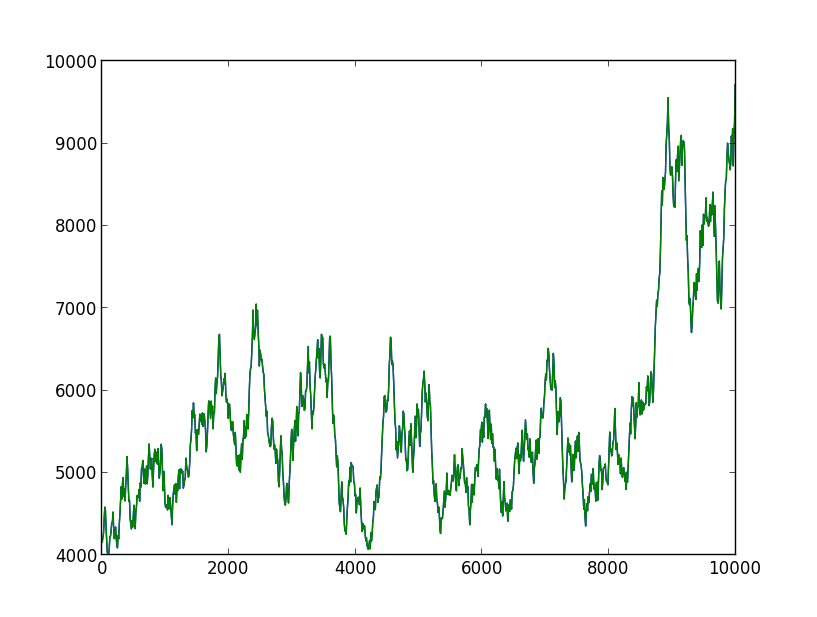
\includegraphics[width=0.7\textwidth]{images/query.png}
    \caption{Query plot}
    \label{fig:query}
\end{figure}

\begin{figure}[h!]
    \centering
    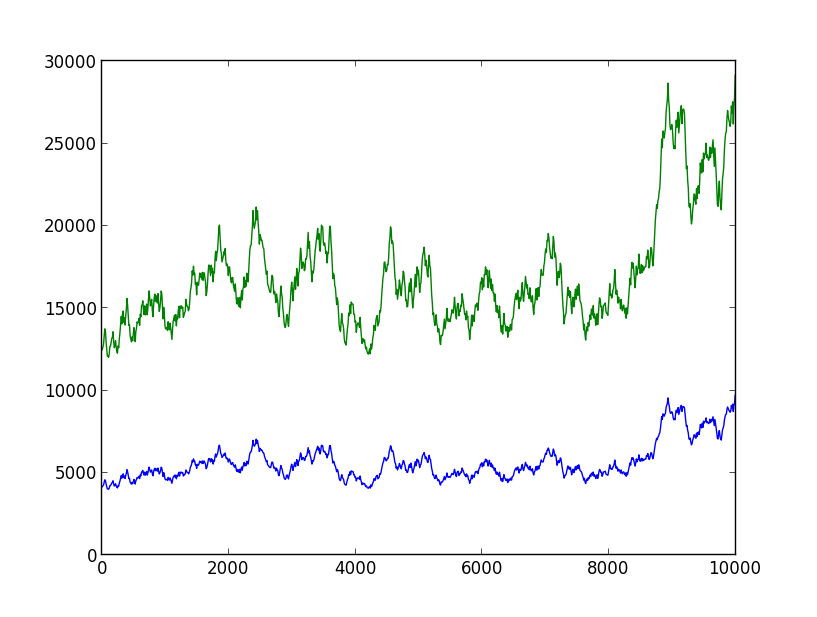
\includegraphics[width=0.7\textwidth]{images/mutant_1.png}
    \caption{First similar plot.  It is a scaling of the original plot by a factor of 3.}
    \label{fig:mutant_1}
\end{figure}

\begin{figure}[h!]
    \centering
    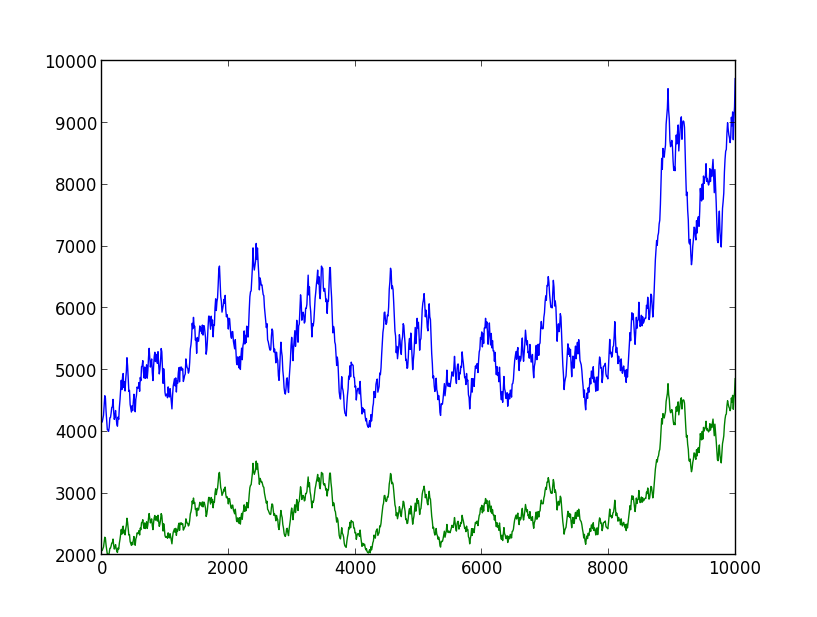
\includegraphics[width=0.7\textwidth]{images/mutant_2.png}
    \caption{Second similar plot.  It is a scaling of the original plot by a factor of 0.5.}
    \label{fig:mutant_2}
\end{figure}

\begin{figure}[h!]
    \centering
    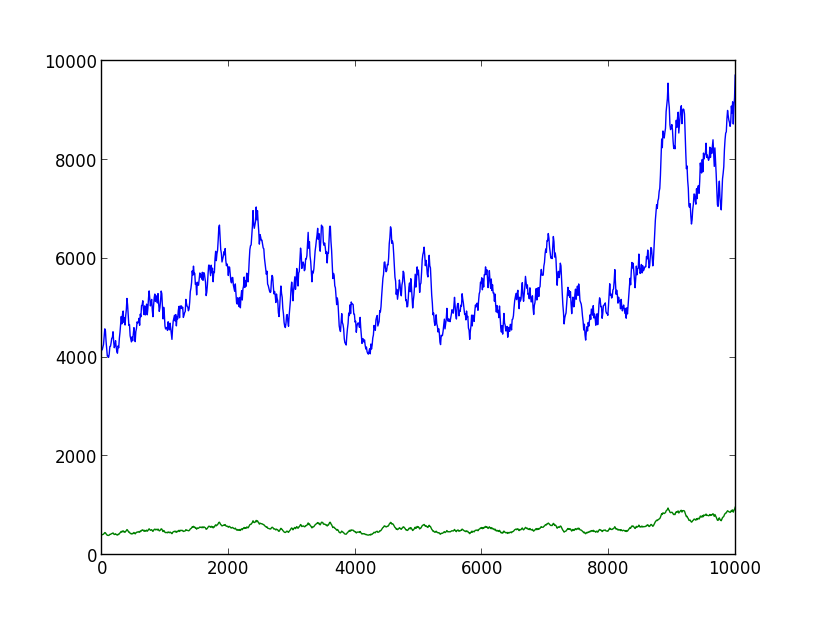
\includegraphics[width=0.7\textwidth]{images/mutant_3.png}
    \caption{Third similar plot.  It is a scaling of the original plot by a factor of 0.1.}
    \label{fig:mutant_3}
\end{figure}

\begin{figure}[h!]
    \centering
    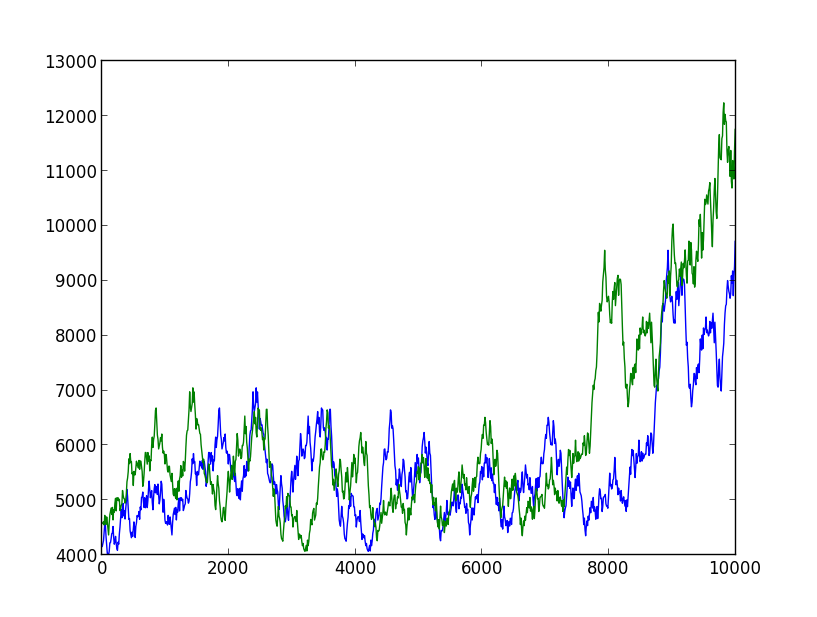
\includegraphics[width=0.7\textwidth]{images/mutant_4.png}
    \caption{Fourth similar plot.  The plot has been shifted left by 10\%.}
    \label{fig:mutant_4}
\end{figure}

\begin{figure}[h!]
    \centering
    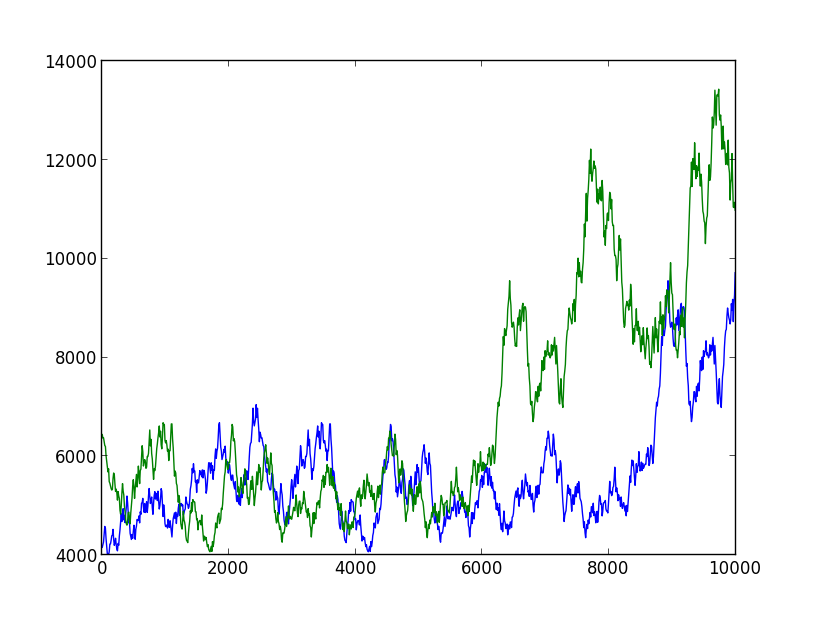
\includegraphics[width=0.7\textwidth]{images/mutant_5.png}
    \caption{Fifth similar plot.  The plot has been shifted left by 25\%.}
    \label{fig:mutant_5}
\end{figure}

\begin{figure}[h!]
    \centering
    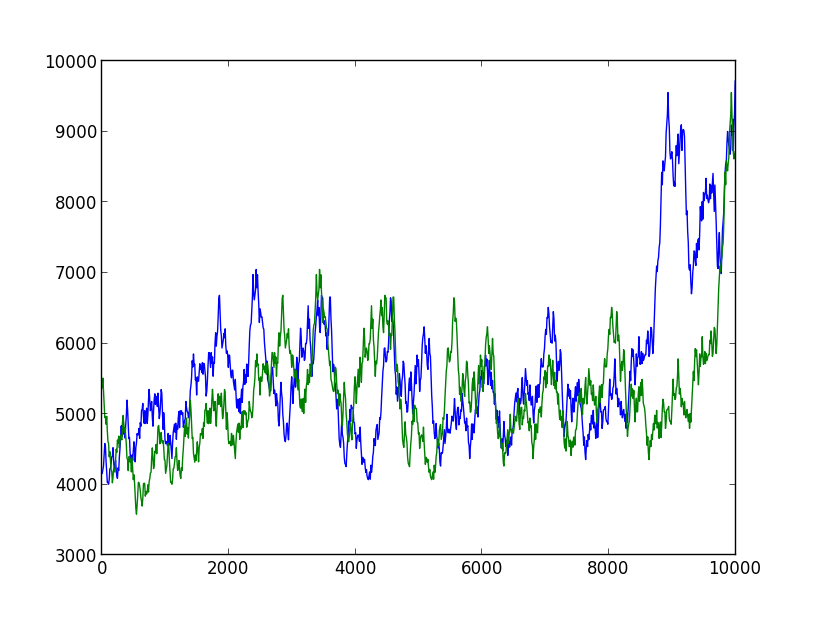
\includegraphics[width=0.7\textwidth]{images/mutant_6.png}
    \caption{Sixth similar plot.  The plot has been shifted right by 10\%.}
    \label{fig:mutant_6}
\end{figure}

\begin{figure}[h!]
    \centering
    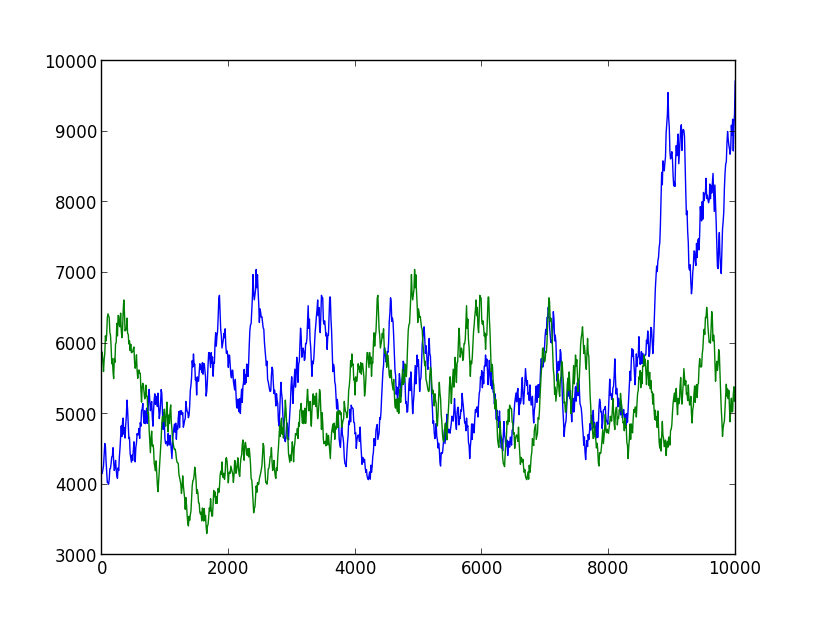
\includegraphics[width=0.7\textwidth]{images/mutant_7.png}
    \caption{Seventh similar plot.  The plot has been shifted right by 25\%.}
    \label{fig:mutant_7}
\end{figure}

\begin{figure}[h!]
    \centering
    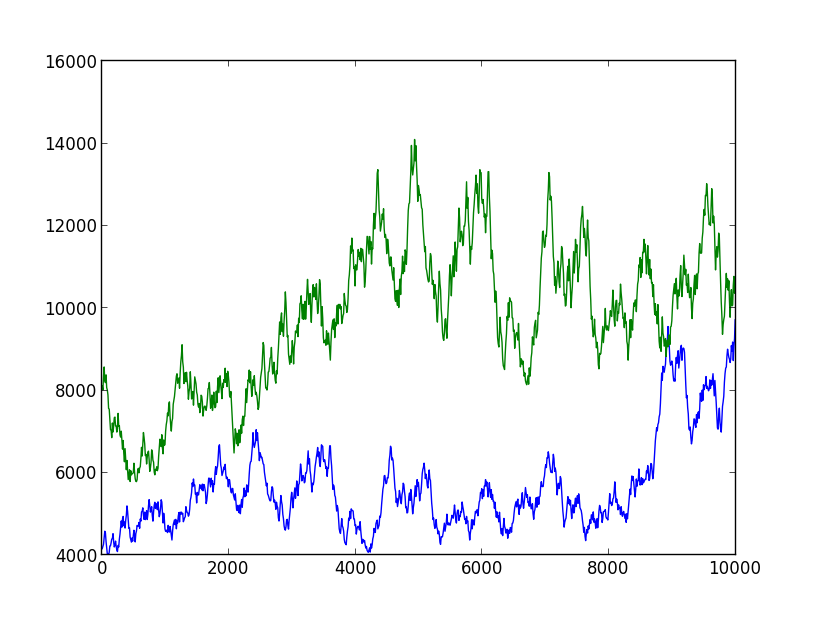
\includegraphics[width=0.7\textwidth]{images/mutant_8.png}
    \caption{Eighth similar plot.  The plot has been shifted right by 25\% and scaled by a factor of 2.}
    \label{fig:mutant_8}
\end{figure}

\begin{figure}[h!]
    \centering
    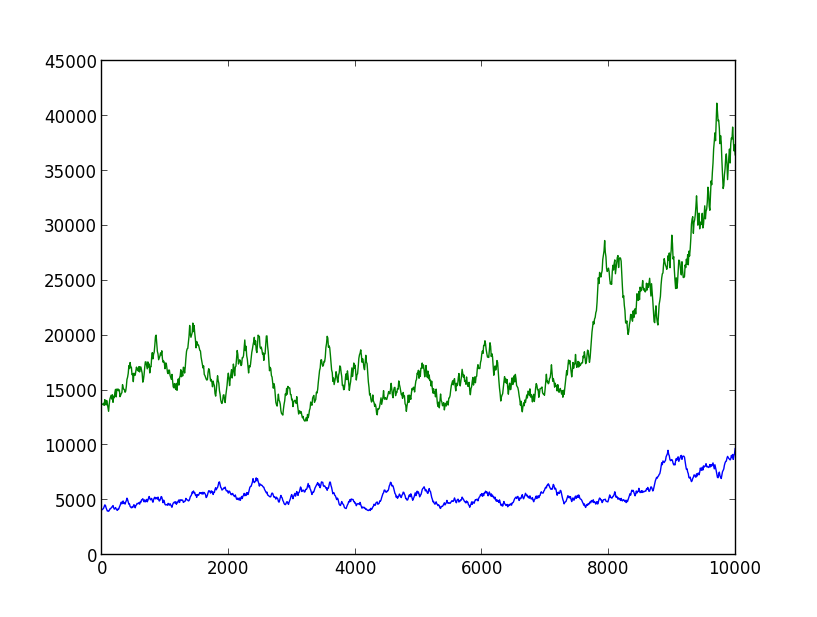
\includegraphics[width=0.7\textwidth]{images/mutant_9.png}
    \caption{Ninth similar plot.  The plot has been shifted left by 10\% and scaled by a factor of 3.}
    \label{fig:mutant_9}
\end{figure}

\begin{figure}[h!]
    \centering
    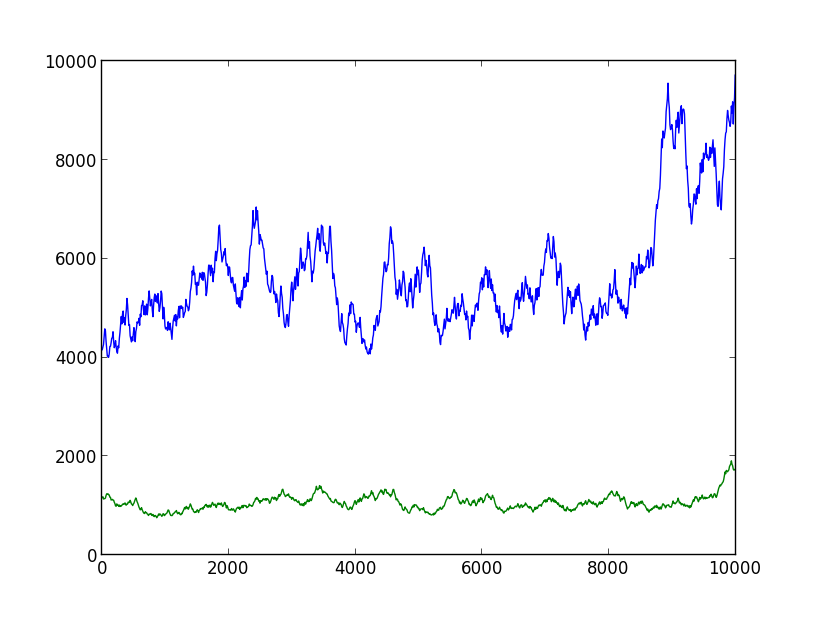
\includegraphics[width=0.7\textwidth]{images/mutant_10.png}
    \caption{Tenth similar plot.  The plot has been shifted right by 10\% and scaled by a factor of 0.2.}
    \label{fig:mutant_10}
\end{figure}

\clearpage

\section{Experiment 1 Graphs}
\label{sec:experiment1}

These are the plots for the results of Experiment 1 in Section~\ref{sec:search_eval}.  In all the graphs the query plot is the blue line and the plot determined to be similar is green.

\begin{figure}[h!]
    \centering
    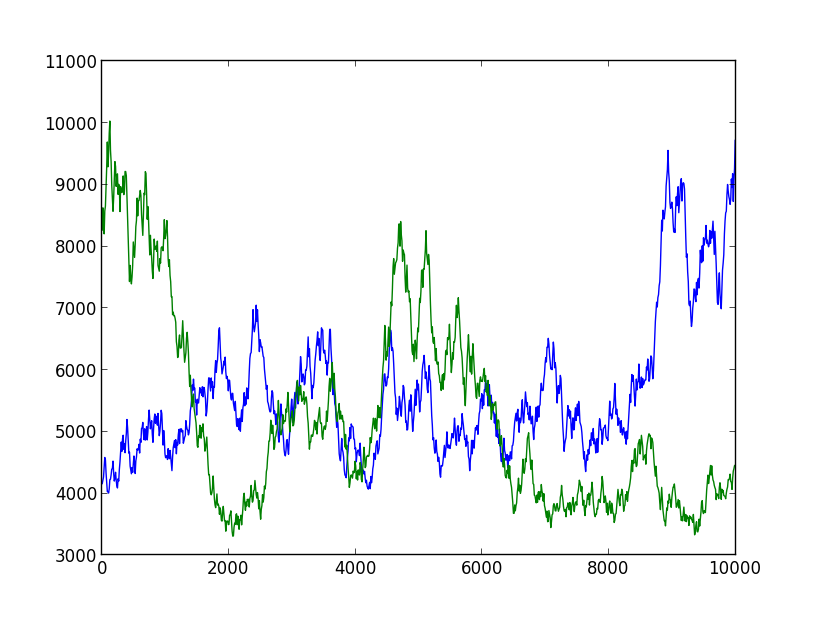
\includegraphics[width=0.7\textwidth]{images/256.png}
    \caption{First similar plot.  Line 256}
    \label{fig:ex1_1}
\end{figure}

\begin{figure}[h!]
    \centering
    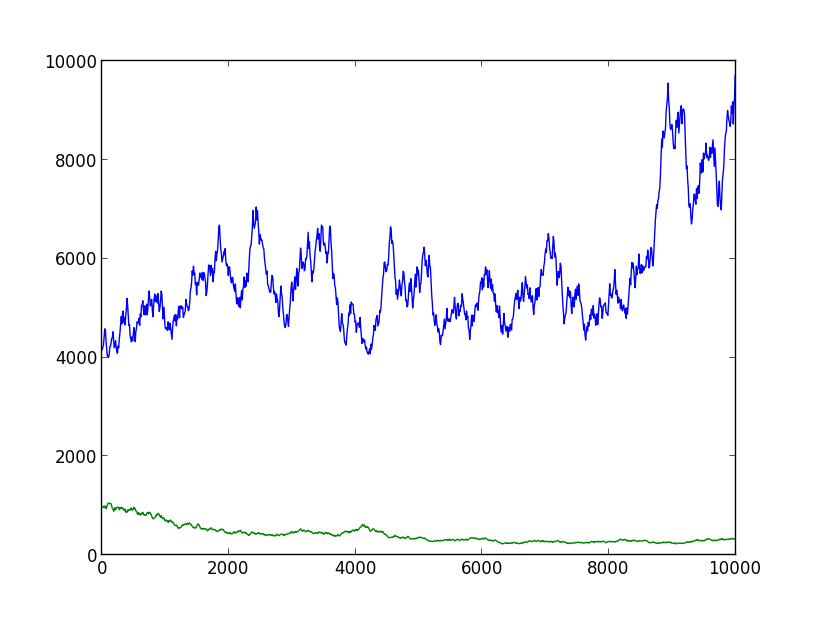
\includegraphics[width=0.7\textwidth]{images/7017.png}
    \caption{Second similar plot.  Line 7017}
    \label{fig:ex1_2}
\end{figure}

\begin{figure}[h!]
    \centering
    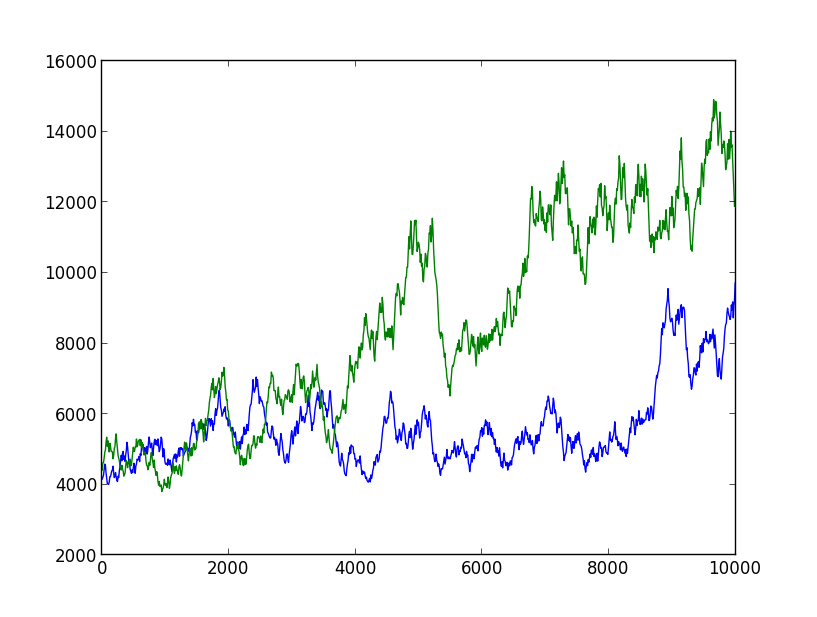
\includegraphics[width=0.7\textwidth]{images/8341.png}
    \caption{Third similar plot.  Line 8341}
    \label{fig:ex1_3}
\end{figure}

\begin{figure}[h!]
    \centering
    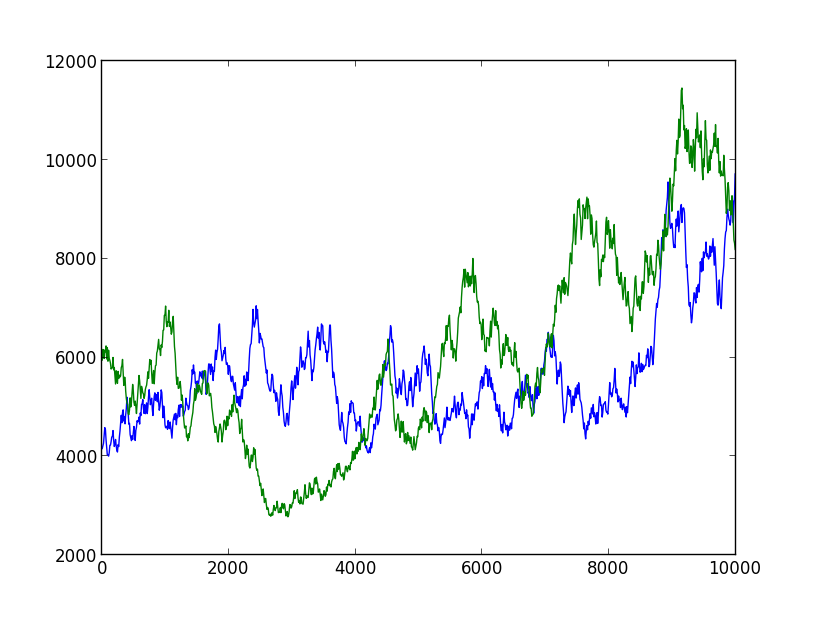
\includegraphics[width=0.7\textwidth]{images/1380.png}
    \caption{Fourth similar plot.  Line 1380}
    \label{fig:ex1_4}
\end{figure}

\begin{figure}[h!]
    \centering
    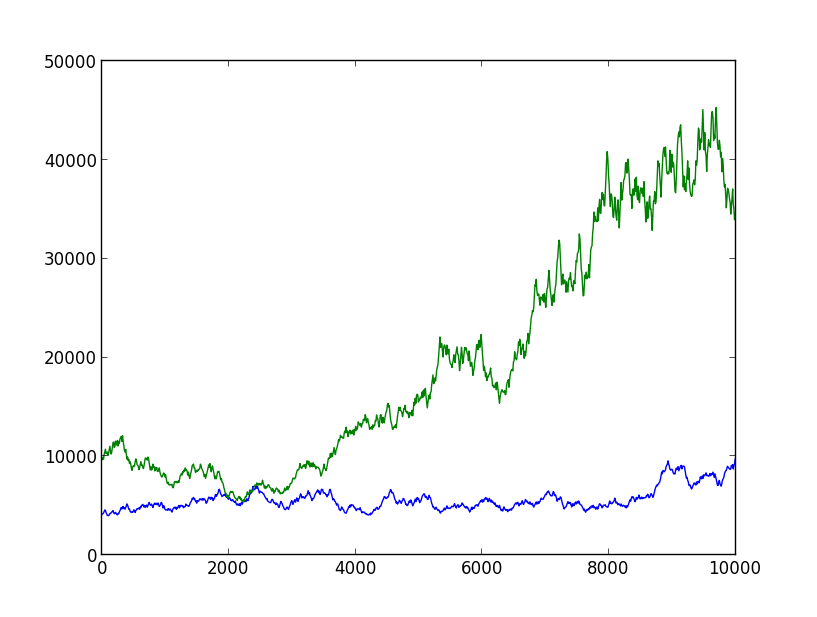
\includegraphics[width=0.7\textwidth]{images/4997.png}
    \caption{Fifth similar plot.  Line 4997}
    \label{fig:ex1_5}
\end{figure}

\begin{figure}[h!]
    \centering
    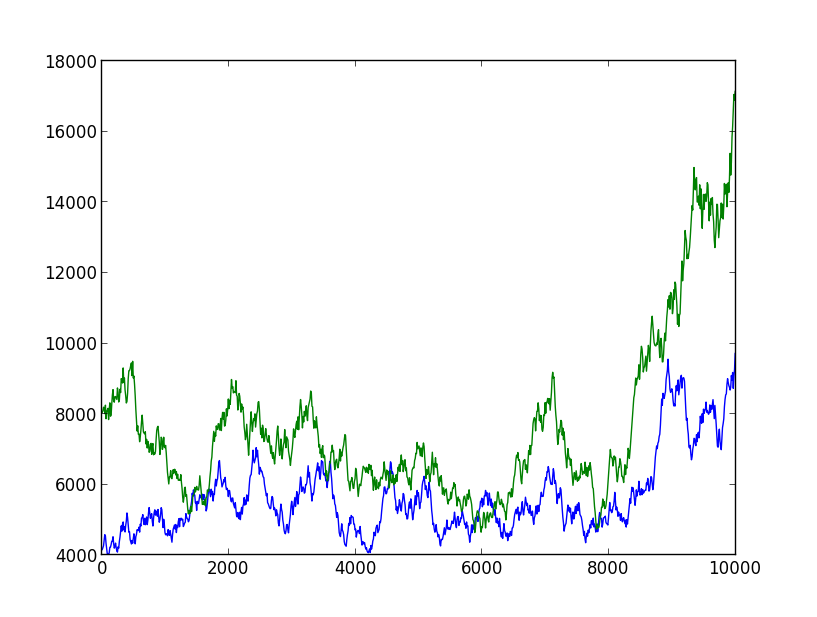
\includegraphics[width=0.7\textwidth]{images/5462.png}
    \caption{Sixth similar plot.  Line 5462}
    \label{fig:ex1_6}
\end{figure}

\begin{figure}[h!]
    \centering
    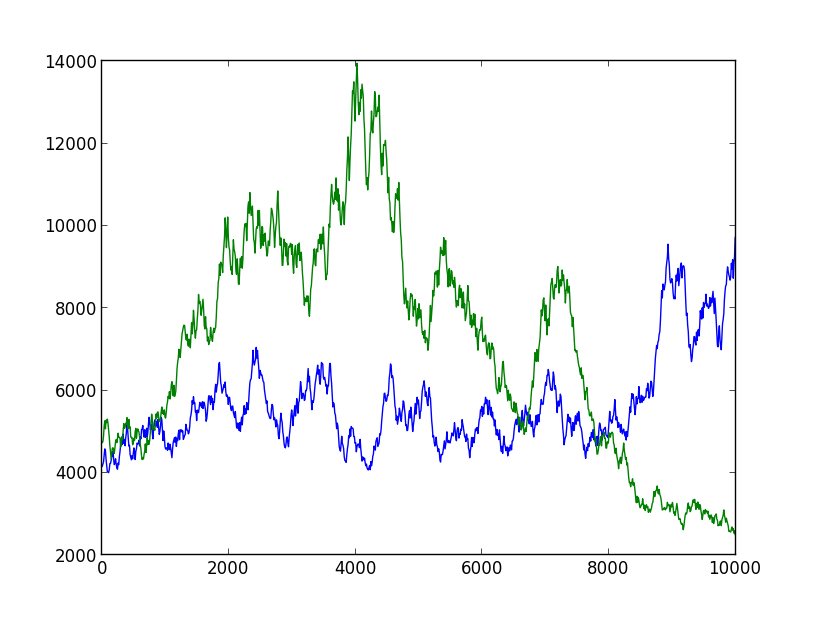
\includegraphics[width=0.7\textwidth]{images/6648.png}
    \caption{Seventh similar plot.  Line 6648}
    \label{fig:ex1_7}
\end{figure}

\begin{figure}[h!]
    \centering
    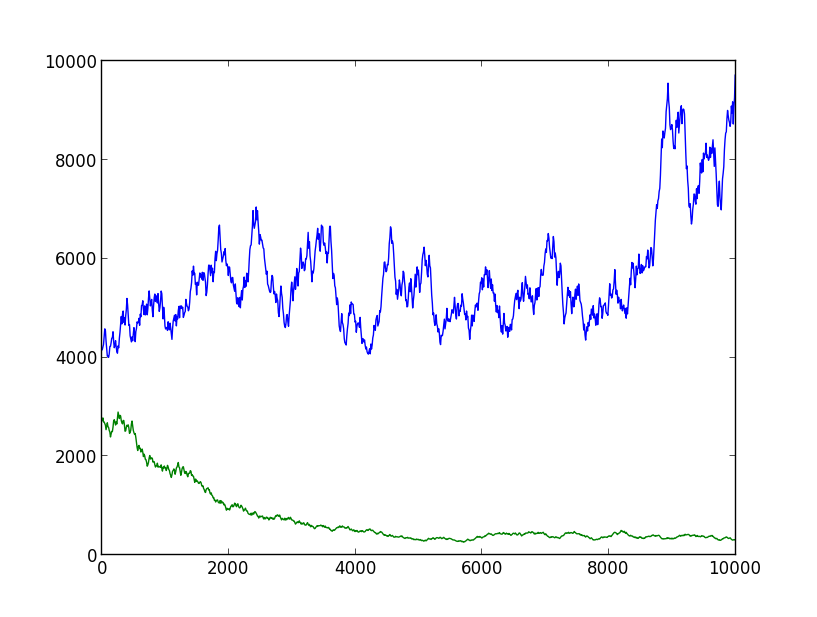
\includegraphics[width=0.7\textwidth]{images/2298.png}
    \caption{Eighth similar plot.  Line 2298}
    \label{fig:ex1_8}
\end{figure}

\begin{figure}[h!]
    \centering
    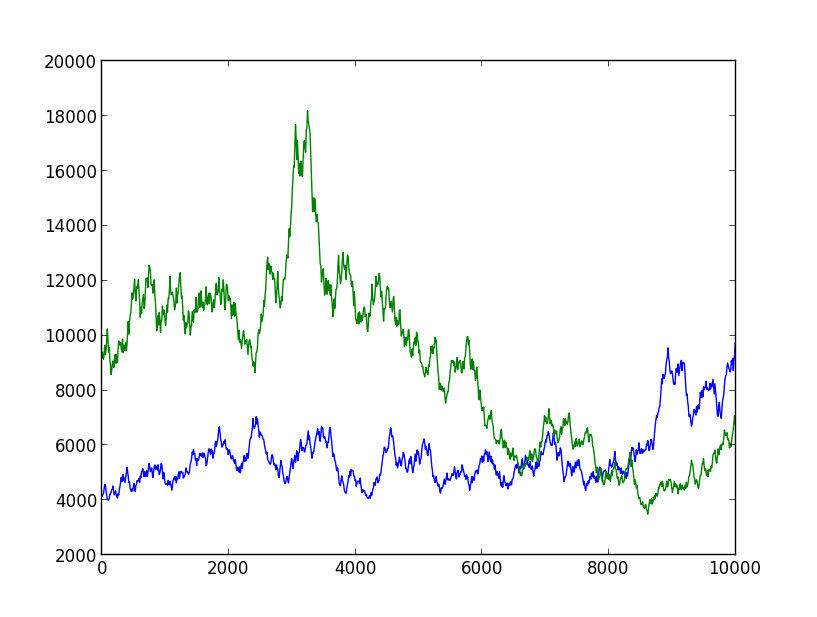
\includegraphics[width=0.7\textwidth]{images/595.png}
    \caption{Ninth similar plot.  Line 595}
    \label{fig:ex1_9}
\end{figure}

\begin{figure}[h!]
    \centering
    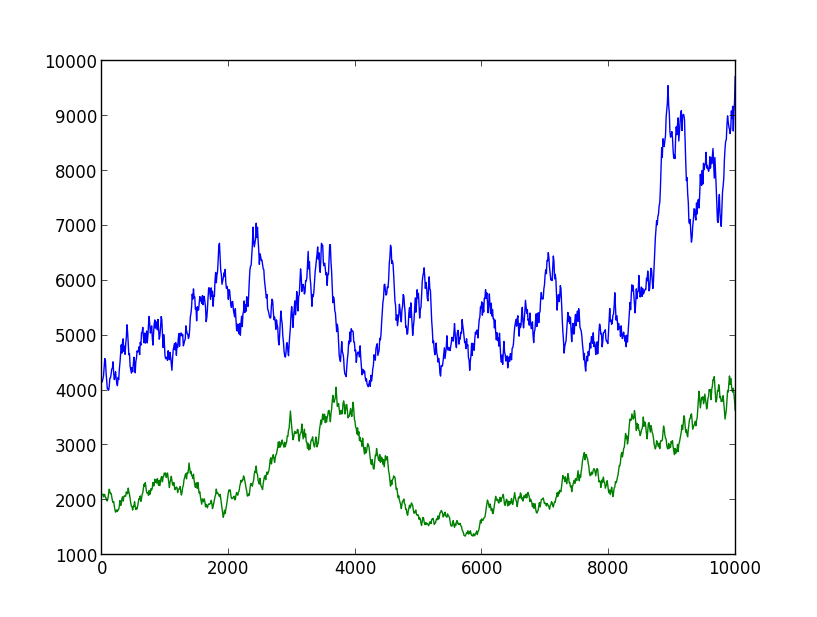
\includegraphics[width=0.7\textwidth]{images/190.png}
    \caption{Tenth similar plot.  Line 190}
    \label{fig:ex1_10}
\end{figure}
